%%%%%%%%%%%%%%%%%%%% ANEXOS / APPENDIX %%%%%%%%%%%%%%%%%%%%%%
\appendix           % appendix starts from here
\appendixpage  		% add a blank page to start the appendix
\addappheadtotoc 	% add appendix to the TOC

\chapter{DAAM Layers Analysis}
\label{chap:appendix-c1}

As part of the study on the attention arrays of DAAM, an exploration was conducted to observe how the attentions from different blocks and epochs aligned, in terms of mIoU, with the objects of the dataset generated. Due to the scope of the project, this line of investigation was left as a direction for future work. This appendix provides a summary of several results from the experiment conducted.

In the original version of DAAM \cite{DAAM}, to construct the heatmap for a token, $D^\mathbb{R}_k$, all attention arrays from different blocks, heads, and timestamps are aggregated (\ref{eq:daam-summing}), meaning that they are summed along the $i, l,$ and $t$ dimensions before aggregation.

To study the variations in attention arrays between different blocks, the mIoU of the objects in the generated dataset was measured without aggregating these dimensions. Specifically, three variants were studied: aggregating only the multi-attention heads ($l$), aggregating the attention heads of each block across all epochs ($l, t$), and aggregating the attention heads and blocks for a single epoch ($l, i$). In other words:

\begin{equation}
\label{eq:daam-not-aggregated}
\begin{gathered}
D_{X,k,t, i}^{\mathbb{R}}[x, y] := \sum_{l} \Tilde{F}_{X, t, k, l}^{(i) \downarrow}[x,y] + \Tilde{F}_{X, t, k, l}^{(i) \uparrow}[x,y]\ , \\
D_{X,k, i}^{\mathbb{R}}[x, y] := \sum_{t, l} \Tilde{F}_{X, t, k, l}^{(i) \downarrow}[x,y] + \Tilde{F}_{X, t, k, l}^{(i) \uparrow}[x,y]\ ,\  \text{and} \\ 
D_{X,k, t}^{\mathbb{R}}[x, y] := \sum_{t, l} \Tilde{F}_{X, t, k, l}^{(i) \downarrow}[x,y] + \Tilde{F}_{X, t, k, l}^{(i) \uparrow}[x,y].
\end{gathered}
\end{equation}

In Figure \ref{fig:heatmap-blocks-epochs-all-05}, we present the preliminary results obtained from this experiment. The main matrix in the figure shows the mIoU scores when evaluating the heatmaps $D_{X,k,t, i}^{\mathbb{R}}$ on the entire generated dataset, including the classes ``car,'' ``person,'' ``traffic light,'' and ``rider.''

The U-Net architecture of Stable Diffusion 2-base comprises 15 blocks with resolutions ranging from 16x16 to 64x64. In the figure, the blocks are arranged vertically, indicating whether they are upsample or downsample blocks. The images are generated through a process involving 31 iterations, represented along the horizontal axis.

A distinct pattern is observed in the blocks. The blocks with higher resolutions, such as 64x64, exhibit better alignment with the objects in the network, resulting in higher mIoU scores. In contrast, the deeper layers show mIoU scores close to 0. This discrepancy may be attributed to the Softmax operation with the other tokens in the text embedding (Eq. \ref{eq:daam-multiscale}) not being effectively activated in lower layers. Further investigation is required, including a visual analysis of the heatmaps from these layers, to precisely determine the cause.

Regarding the aggregation of a complete block within a single epoch (additional row on top of the matrix in Figure \ref{fig:heatmap-blocks-epochs-all-05}), it is noticeable that the attention maps from the first and last epochs exhibit poorer alignment with the ground truth described by the token. This discrepancy may stem from the fact that, in the early epochs, the latent space is filled with noise, and the object has not yet fully formed. Similarly, in the last epochs, the attention maps may not prioritize the object as much, since the images are already close to their final state.


\begin{figure}
    \centering
    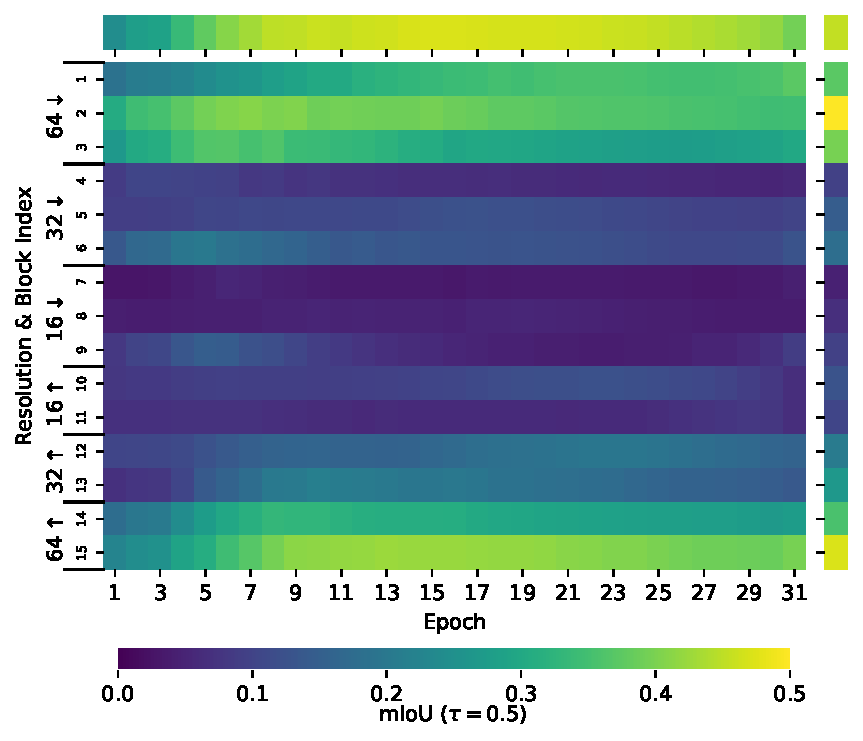
\includegraphics[width=0.8\columnwidth]{img/4-experiments/heatmap_all_05.pdf}
    \caption[Heatmap Analysis of DAAM Blocks and Epochs.]{Heatmap Analysis of DAAM Blocks and Epochs. The matrix illustrates the mIoU scores obtained from evaluating the heatmaps $D_{X,k,t, i}^{\mathbb{R}}$ on the generated dataset for different blocks and epochs. The vertical axis represents the U-Net blocks, ordered by their location in the U-net (downsample to upsample), while the horizontal axis corresponds to the epochs during the generation process. The additional top row shows the mIoU scores when aggregating all blocks in one epoch, and the additional right column displays the mIoU scores when aggregating a block across all epochs. The results reveal the variation in alignment between attention maps and ground truth objects across different blocks, epochs, and aggregation strategies.}
    \label{fig:heatmap-blocks-epochs-all-05}
\end{figure}

After examining the results disaggregated by layers in Figure \ref{fig:heatmap-blocks-epochs-all-05}, it becomes evident that aggregating layers leads to higher mIoU scores for the resulting heatmaps. This observation suggests that different blocks contain complementary information, and choosing a single block would result in the loss of object-related information during segmentation. To assess the information shared among blocks, linear correlations were calculated between the aggregated heatmaps across all epochs ($D_{X,k, i}^{\mathbb{R}}$, subfigure \ref{fig:block-correlation}) and across all blocks ($D_{X,k, t}^{\mathbb{R}}$, subfigure \ref{fig:block-correlation}).

In the block correlation analysis (subfigure \ref{fig:block-correlation}), it can be observed that blocks with higher resolutions (64x64 and 32x32) exhibit significant linear correlations. The strong correlation among the 64x64 blocks aligns with the high mIoU scores observed in the previous figure (\ref{fig:heatmap-blocks-epochs-all-05}). If these blocks are activated in the regions where the objects are located (resulting in high mIoU scores), they will be activated in the same regions, thus explaining their linear correlation. However, the 32x32 blocks require further analysis, as they have low mIoU scores with the objects in the dataset but still exhibit moderate correlations (around 0.6) among themselves and with the 64x64 blocks. A more in-depth study is needed to determine the regions activated by these blocks.

Regarding the linear correlations between epochs (subfigure \ref{subfig:epoch-correlation}), a clear pattern emerges: heatmaps from nearby epochs are highly similar. This suggests that the focus of attention gradually shifts during the process, attending to different parts of the image. In the original work of DAAM \cite{DAAM}, a brief ablation study was conducted, demonstrating that removing the attention maps from the first and second halves of the epochs resulted in lower mIoU scores. Although a more detailed analysis is required, this suggests that the attention maps across epochs are complementary, and aggregating all of them provides a more comprehensive mask for object segmentation.

It is worth noting that in the figure, the scale used to represent correlations ranges from 0 to 1 (rather than -1 to 1). This is because no results exhibited correlations below 0.

\begin{figure}
\centering
\begin{subfigure}{0.4452\columnwidth}
    \centering
    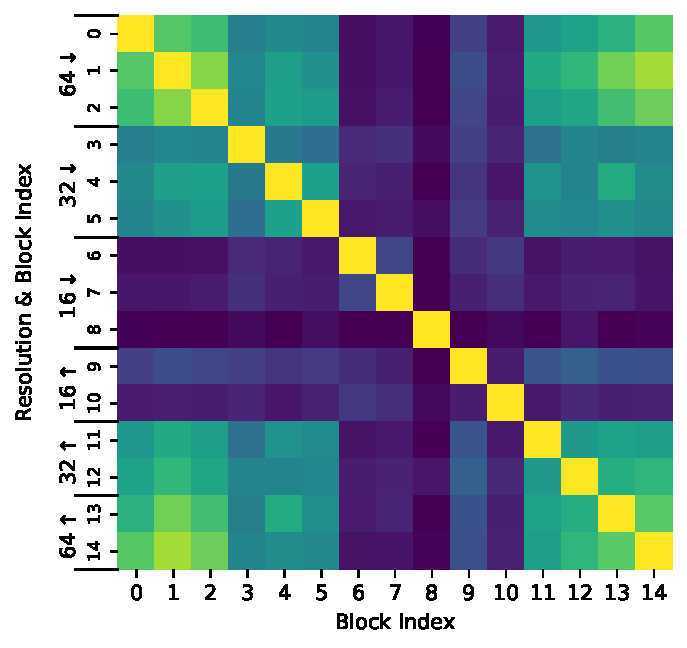
\includegraphics[width=\columnwidth]{img/4-experiments/heatmap_correlations.pdf}
    \caption{Block correlations}
    \label{fig:block-correlation}
\end{subfigure}
\begin{subfigure}{0.545\columnwidth}
    \centering
    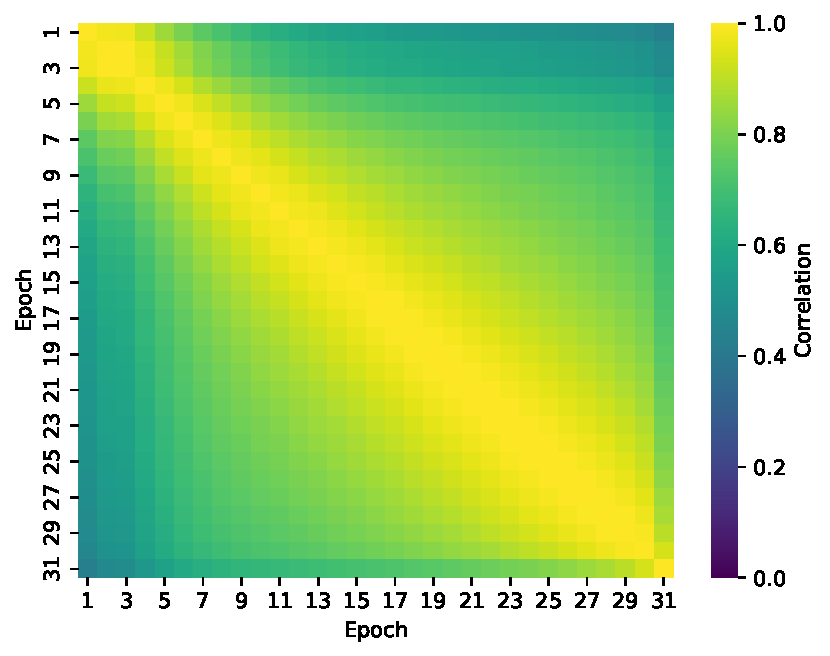
\includegraphics[width=\columnwidth]{img/4-experiments/epoch_correlations.pdf}
    \caption{Epoch correlations}
    \label{subfig:epoch-correlation}
\end{subfigure}
    \caption[Linear correlation analysis of block and epoch heatmaps]{Linear correlations among different elements in the DAAM heatmaps. Subfigure \ref{fig:block-correlation} shows the linear correlations between the aggregated heatmaps across all epochs ($D_{X,k, i}^{\mathbb{R}}$) for each block, while Subfigure \ref{subfig:epoch-correlation} presents the linear correlations between the aggregated heatmaps across all blocks ($D_{X,k, t}^{\mathbb{R}}$) for each epoch. The color scale represents the correlation values, ranging from 0 to 1, where 0 indicates no correlation and 1 represents a perfect linear correlation.}
    \label{fig:correlations}
\end{figure}

%%%%%%%%%%%%%%%%% Text prompt optimization
\chapter{Text prompt optimization}
\label{chap:appendix-text-prompt}

This appendix includes additional figures related to the DAAM optimization experiment described in Section \ref{sec:experiment-optimization}.

Specifically, it presents the loss vs epoch curves for the optimization of Linear DAAMs with different numbers of training samples (Figure \ref{fig:apendix-loss-curves}) and for the non-linear DAAM optimization (Figure \ref{fig:miou-optimized-ious-daam}).

For the optimization process, we conducted 500 epochs, saving checkpoints of the embedding to be optimized every 30 steps. The final epoch, which yielded the best results in terms of mIoU on the test set, was selected. A learning rate of $lr=3$ was utilized.

Additionally, IoU vs threshold curves for the training with different numbers of training samples are included (Figure \ref{fig:apendix-loss-curves}), as well as examples excluded from the main body of the work due to their similar results (Figure \ref{fig:dataset-examples-daam-optimized}).

The optimization experiments were conducted on an Apple M1 Max laptop with 64GB of memory and a GPU with 32 cores. The optimization process required approximately 0.5 seconds per epoch per image.

\begin{figure}
\centering
  % First column
  \begin{subfigure}{0.24\columnwidth}
   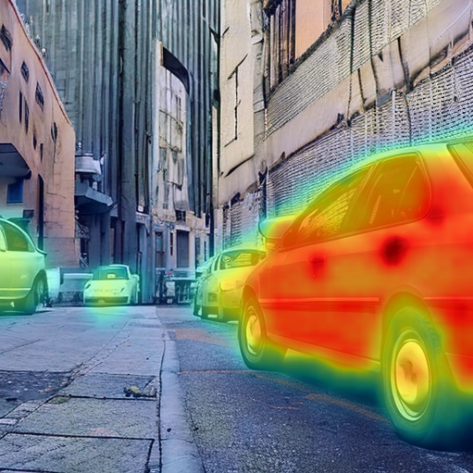
\includegraphics[width=\columnwidth]{img/4-experiments/dataset_example_daam_heatmap_car-full-optimized.png}
   \caption{Car}
   \label{subfig:dataset-example-car-daam-optimized}
  \end{subfigure}
  \begin{subfigure}{0.24\columnwidth}
   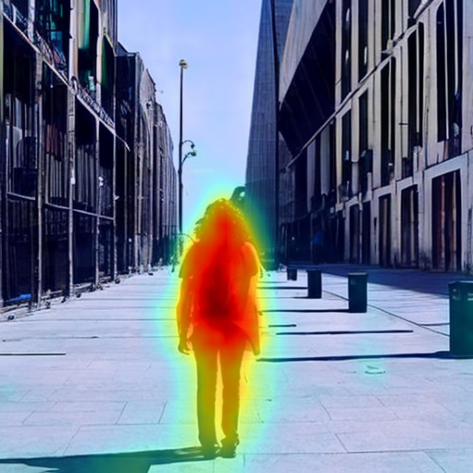
\includegraphics[width=\columnwidth]{img/4-experiments/dataset_example_daam_heatmap_person-full-optimized.png}
   \caption{Person}
   \label{subfig:dataset-example-person-daam-optimized}
  \end{subfigure}
  \begin{subfigure}{0.24\columnwidth}
   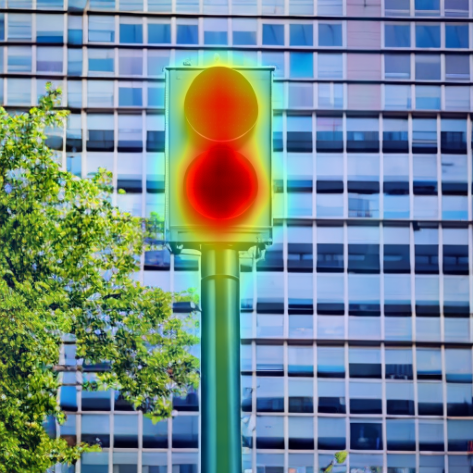
\includegraphics[width=\columnwidth]{img/4-experiments/dataset_example_daam_heatmap_traffic light-full-optimized.png}
   \caption{Traffic light}
   \label{subfig:dataset-example-traffic-daam-optimized}
  \end{subfigure}
  \begin{subfigure}{0.24\columnwidth}
   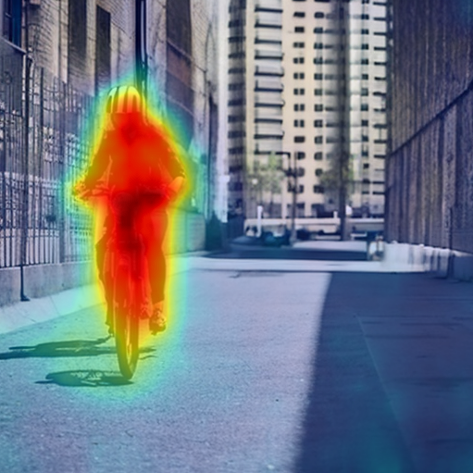
\includegraphics[width=\columnwidth]{img/4-experiments/dataset_example_daam_heatmap_rider-full-optimized.png}
   \caption{Rider}
   \label{subfig:dataset-example-rider-daam-optimized}
  \end{subfigure}
  \caption[Examples of DAAM-generated soft heatmaps optimized]{Examples of DAAM-generated soft heatmaps with a optimized prompt. Each subfigure displays an image for each class with the overlayed soft heatmap generated using DAAM.}
  \label{fig:dataset-examples-daam-optimized}
  \end{figure}


\begin{figure}
\centering
\begin{subfigure}{0.9\columnwidth}
    \centering
    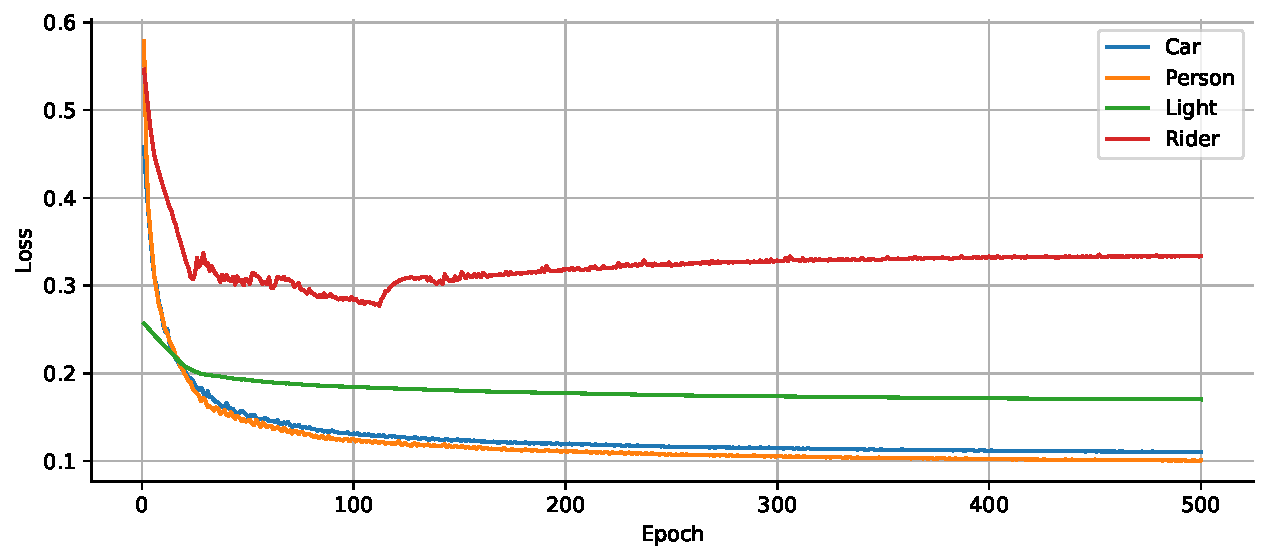
\includegraphics[width=\columnwidth]{img/6-appendix/optimization-curve-1-images.pdf}
    \label{fig:apendix-loss-curves-1-image}
    \caption{Optimization with 1 image per class}
\end{subfigure}
\begin{subfigure}{0.9\columnwidth}
    \centering
    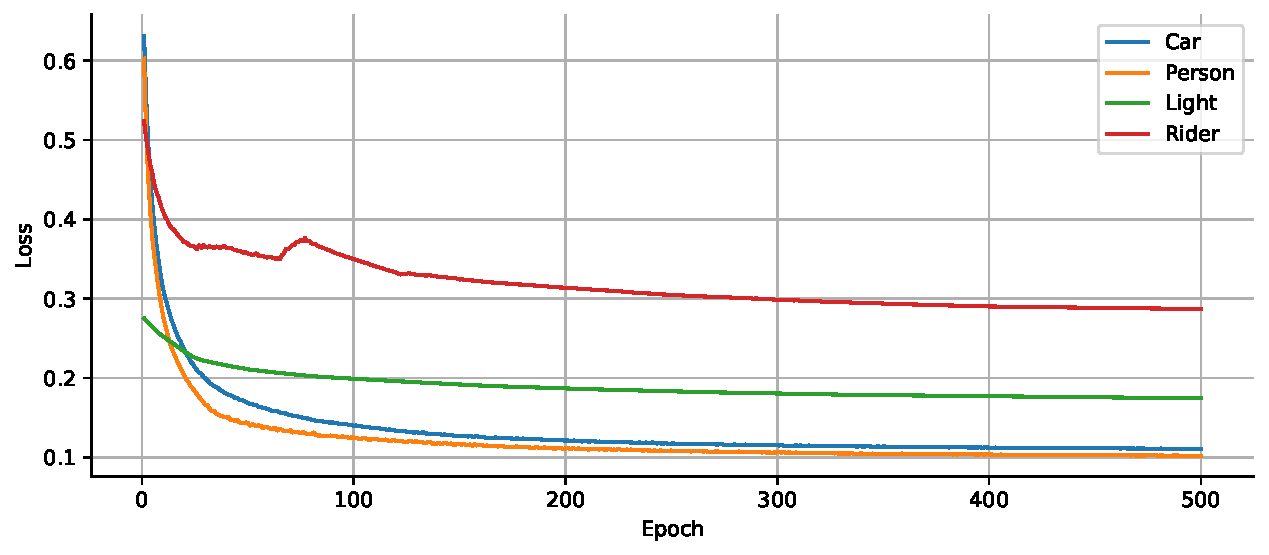
\includegraphics[width=\columnwidth]{img/6-appendix/optimization-curve-2-images.pdf}
    \label{fig:apendix-loss-curves-2-image}
    \caption{Optimization with 2 images per class}
\end{subfigure}
\begin{subfigure}{0.9\columnwidth}
    \centering
    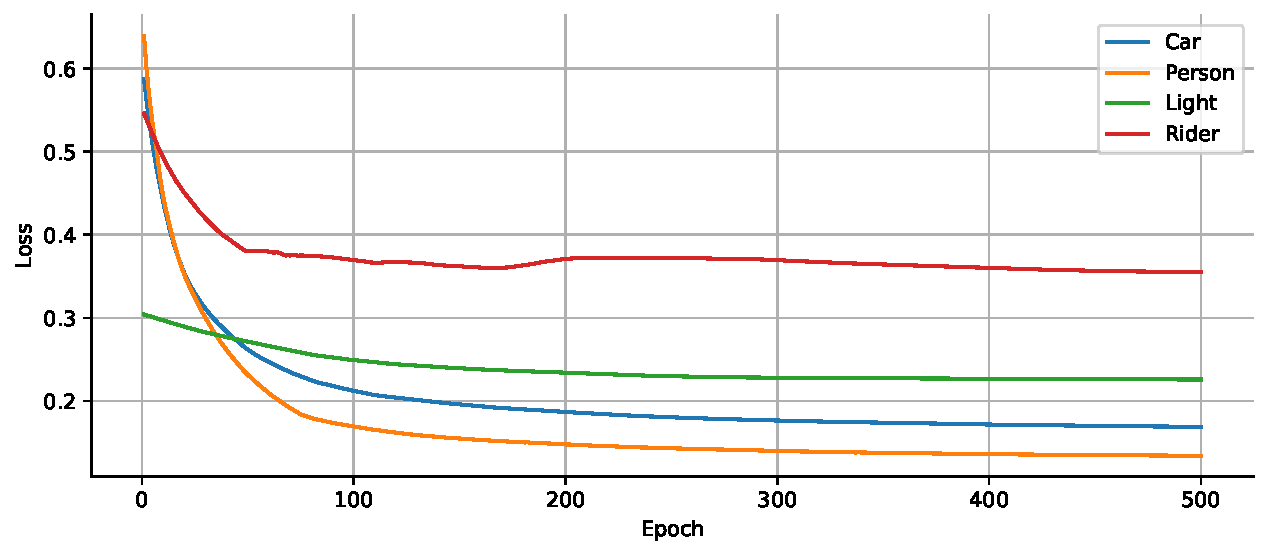
\includegraphics[width=\columnwidth]{img/6-appendix/optimization-curve-5-images.pdf}
    \label{fig:apendix-loss-curves-5-image}
    \caption{Optimization with 5 images per class}
\end{subfigure}
    \caption[Linear DAAM optimization loss curves]{Linear DAAM optimization loss curves}
    \label{fig:apendix-loss-curves}
\end{figure}


\begin{figure}
    \centering
    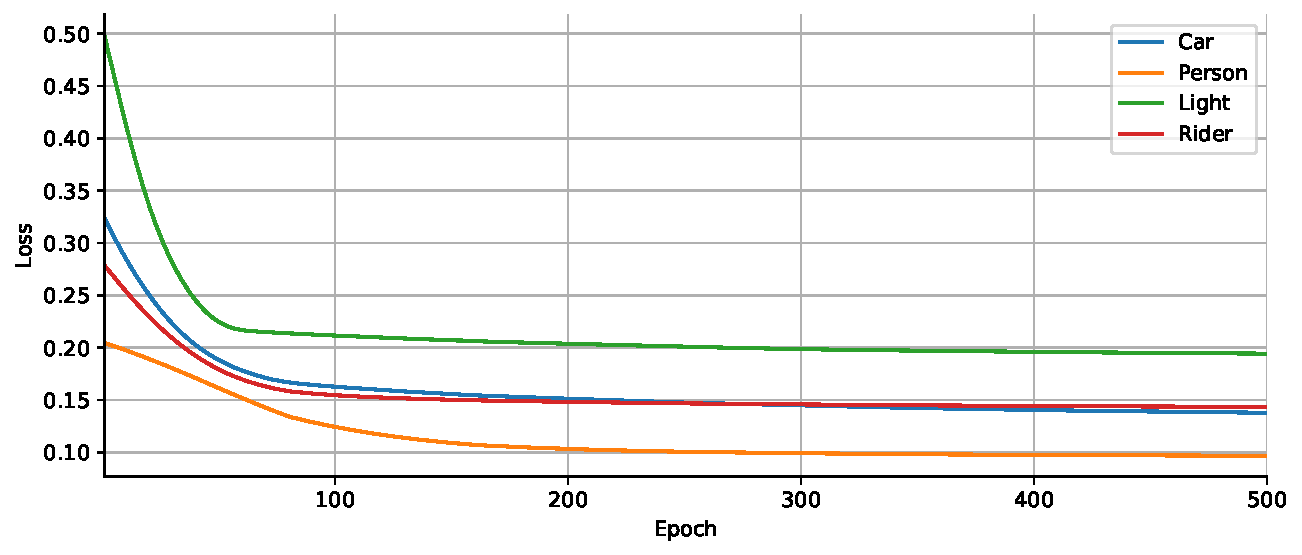
\includegraphics[width=0.8\columnwidth]{img/6-appendix/optimization-curve-2-images-daam.pdf}
    \caption[DAAM optimization]{DAAM optimization loss curves with 2 images as train. The token embedding optimized contains 2 words: The main token (car/Person/Light/Rider) and a background token (with the complementary target mask).}
    \label{fig:miou-optimized-ious-daam}
\end{figure}


\begin{figure}
    \centering
    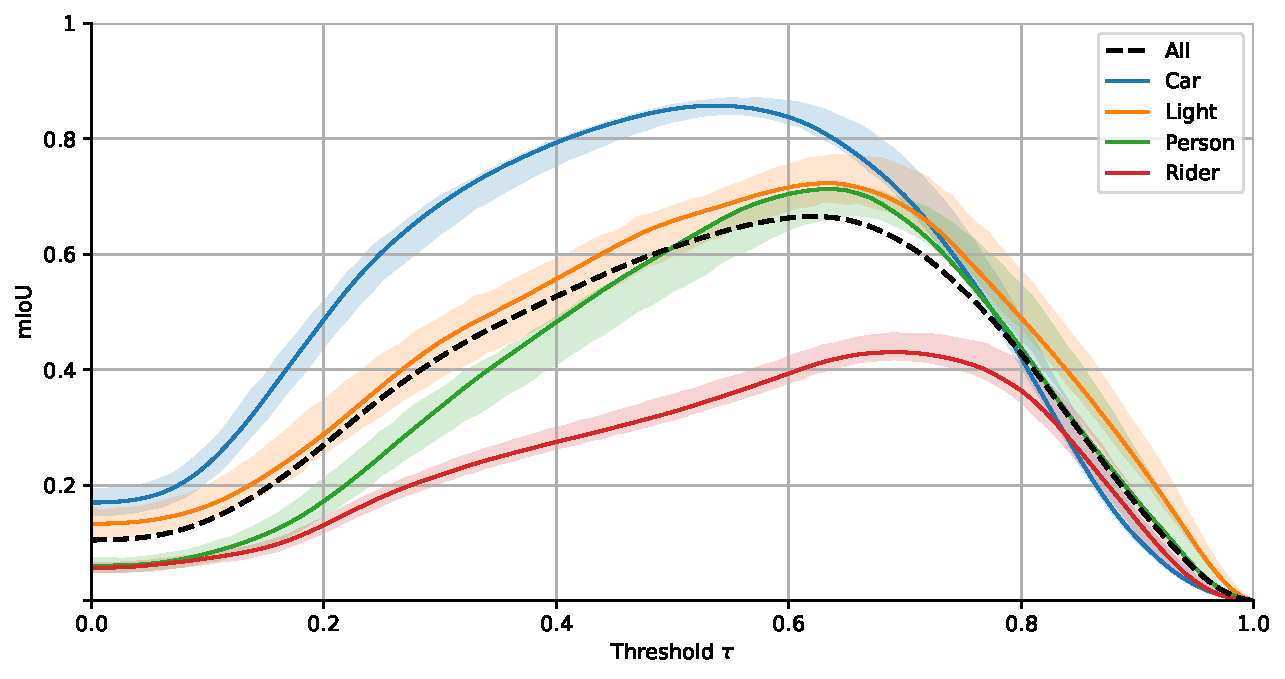
\includegraphics[width=1\columnwidth]{img/4-experiments/full-heatmap-optimized-iou-2-500-test-large.pdf}
    \caption[Optimized DAAM mIoU curves]{Optimized DAAM (Non-linear Open Vocabulary DAAM), mIoU vs threshold curves. Performance of the test set}
    \label{fig:miou-class-curves-daam-optimized}
\end{figure}


%%%%%%%%%%%%%%%%%%% Curves
\begin{figure}
\centering
  % First column
  \begin{subfigure}{0.49\columnwidth}
   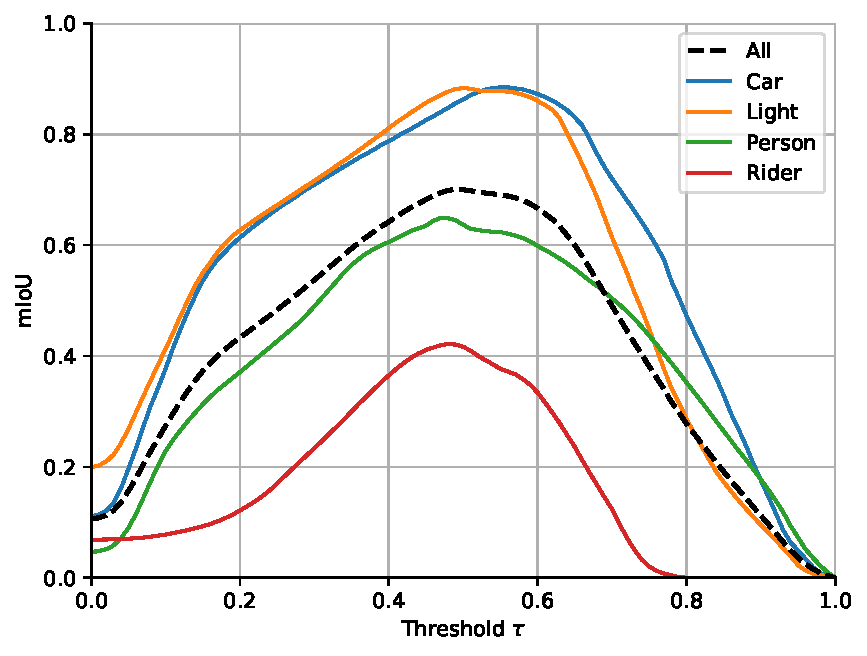
\includegraphics[width=\columnwidth]{img/4-experiments/heatmap-optimized-iou-1-300-train.pdf}
   \caption{Train (1 sample / class)}
   \label{fig:miou-optimized-ious-train-1}
  \end{subfigure}
  \begin{subfigure}{0.49\columnwidth}
   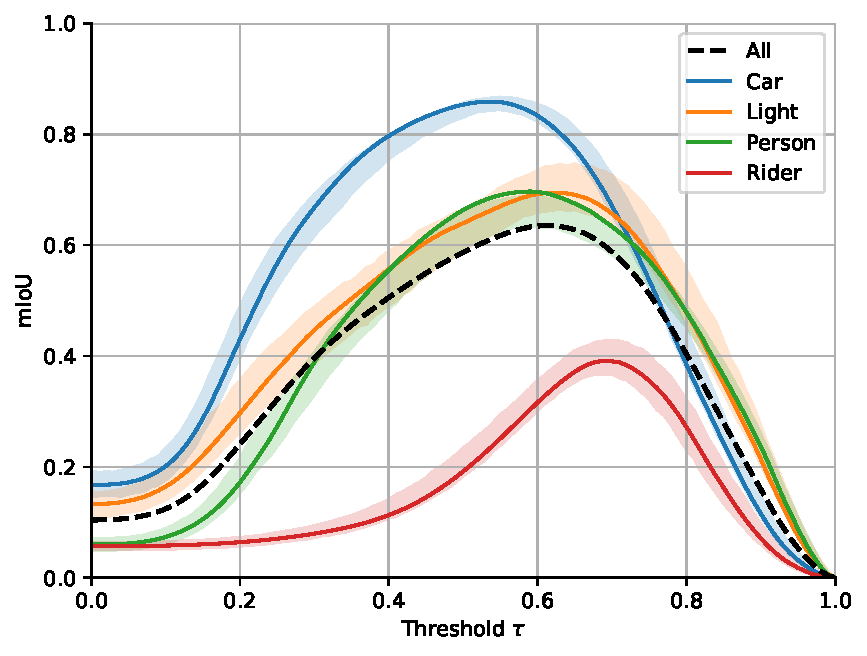
\includegraphics[width=\columnwidth]{img/4-experiments/heatmap-optimized-iou-1-300-test.pdf}
   \caption{Test (1 sample / class)}
   \label{fig:miou-optimized-ious-test-1}
  \end{subfigure}
  % Second column
  \begin{subfigure}{0.49\columnwidth}
   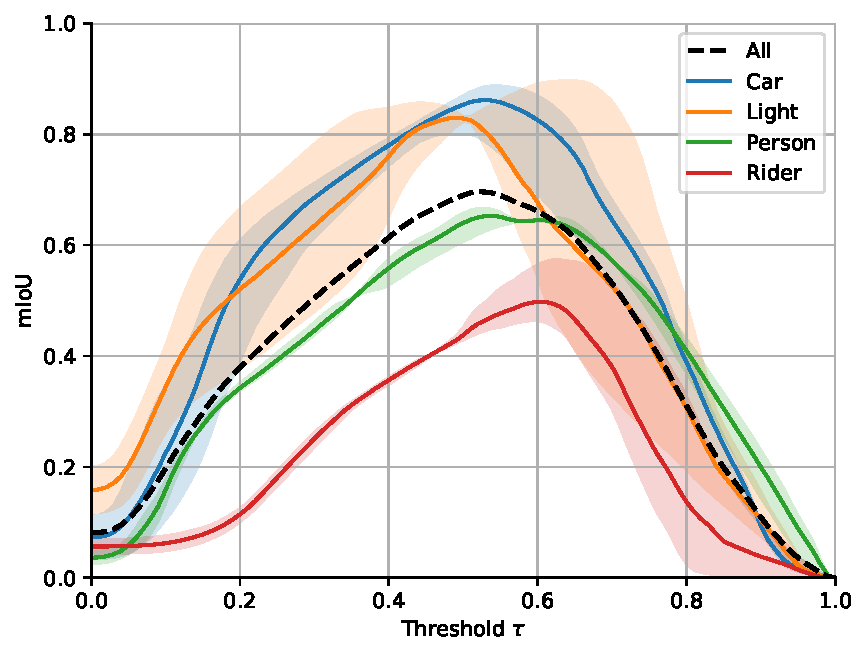
\includegraphics[width=\columnwidth]{img/4-experiments/heatmap-optimized-iou-2-300-train.pdf}
   \caption{Train (2 samples / class)}
   \label{fig:miou-optimized-ious-train-2}
  \end{subfigure}
  \begin{subfigure}{0.49\columnwidth}
   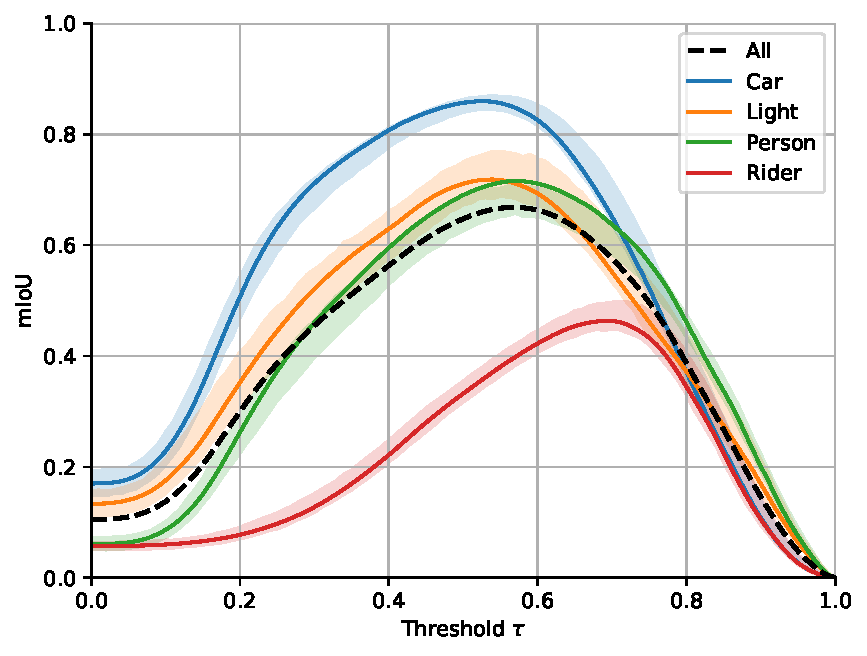
\includegraphics[width=\columnwidth]{img/4-experiments/heatmap-optimized-iou-2-300-test.pdf}
   \caption{Test (2 samples / class)}
   \label{fig:miou-optimized-ious-test-2}
  \end{subfigure}
  % Third column
  \begin{subfigure}{0.49\columnwidth}
   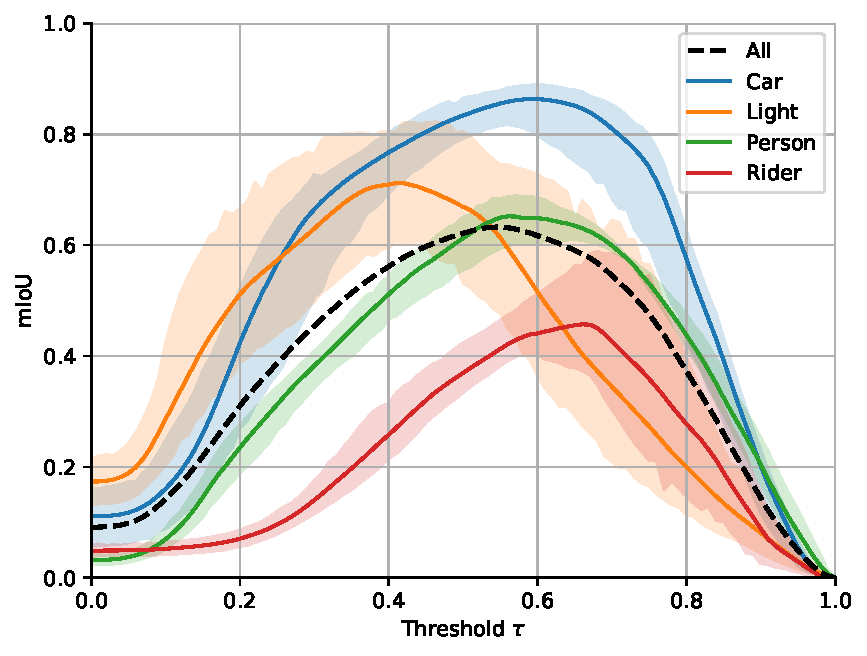
\includegraphics[width=\columnwidth]{img/4-experiments/heatmap-optimized-iou-5-300-train.pdf}
   \caption{Train (5 samples / class)}
   \label{fig:miou-optimized-ious-train-5}
  \end{subfigure}
  \begin{subfigure}{0.49\columnwidth}
   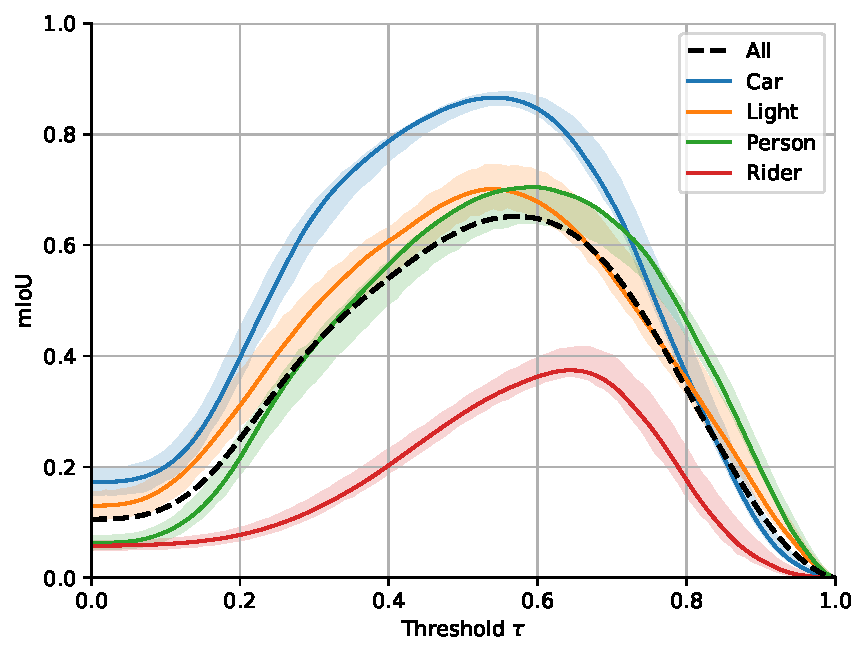
\includegraphics[width=\columnwidth]{img/4-experiments/heatmap-optimized-iou-5-300-test.pdf}
   \caption{Test (5 samples / class)}
   \label{fig:miou-optimized-ious-test-5}
  \end{subfigure}
  
  \caption[Linear DAAM with Optimized prompt IoU]{Linear DAAM with Optimized prompt IoU}
  \label{fig:miou-optimized-ious}
  \end{figure}



%%%%%%%%%%%% DATASET
\chapter{Dataset}
\label{chap:appendix-text-dataset}
 
This appendix includes the 200 images of the dataset used in the experiments, which were generated synthetically for this purpose. The dataset consists of four classes: "car" (Figs. \ref{fig:dataset-car}), "person" (Figs. \ref{fig:dataset-person}), "traffic light" (Figs. \ref{fig:dataset-traffic}), and "rider" (Figs. \ref{fig:dataset-rider}).

The images were generated using the Stable Diffusion 2-base architecture trained by StabilityAI \footnote{\href{https://huggingface.co/stabilityai/stable-diffusion-2-base}{https://huggingface.co/stabilityai/stable-diffusion-2-base}, accessed June 2023}. Specifically, revision d28fc8045793886e512c5389771d3b3d560f9575 of the model was utilized.

To produce images with different outcomes while using the same text prompt per class, a random seed was varied. A total of 50 numbers were randomly generated and used as seeds to generate the images for each of the four classes. The same set of seeds was applied to different classes intentionally to maintain similar spatial complexity across classes and minimize external factors that could influence the results. Images generated with the same seed (and therefore initialized with the same random noise vector) tend to exhibit similar spatial compositions. In the dataset images, one can observe how images in the same position within the image matrix of their class share similarities with images from other classes, occasionally featuring common elements such as a specific building or even a watermark.

The dataset was generated using an Apple M1 Max laptop with 64GB of memory and a GPU with 32 cores. The generation process required approximately 30 seconds per image.

\begin{figure}
    \centering
    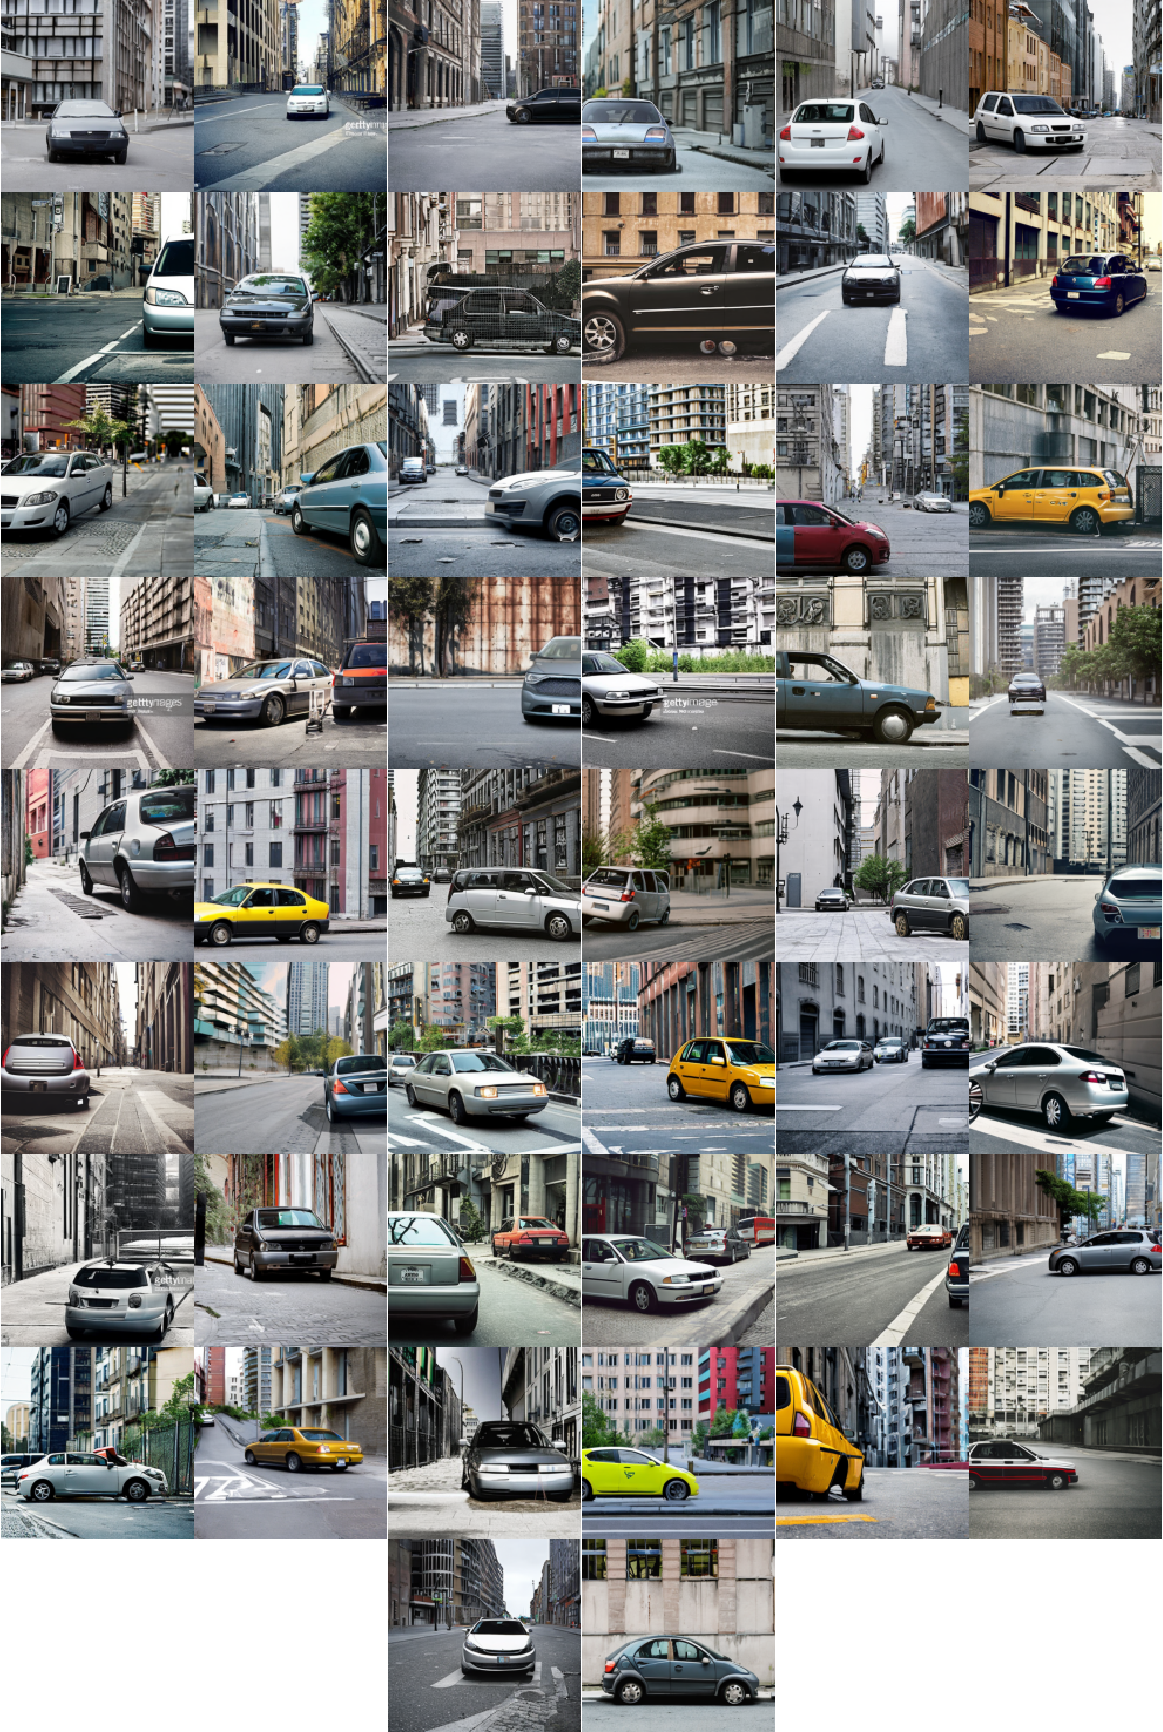
\includegraphics[width=1\columnwidth]{img/6-appendix/dataset_example_car.pdf}
    \caption[Dataset images 1-50]{Images 1-50. Class ``car''. Images generated with the prompt ``A car in an urban environment`` varying the random seed.}
    \label{fig:dataset-car}
\end{figure}


\begin{figure}
    \centering
    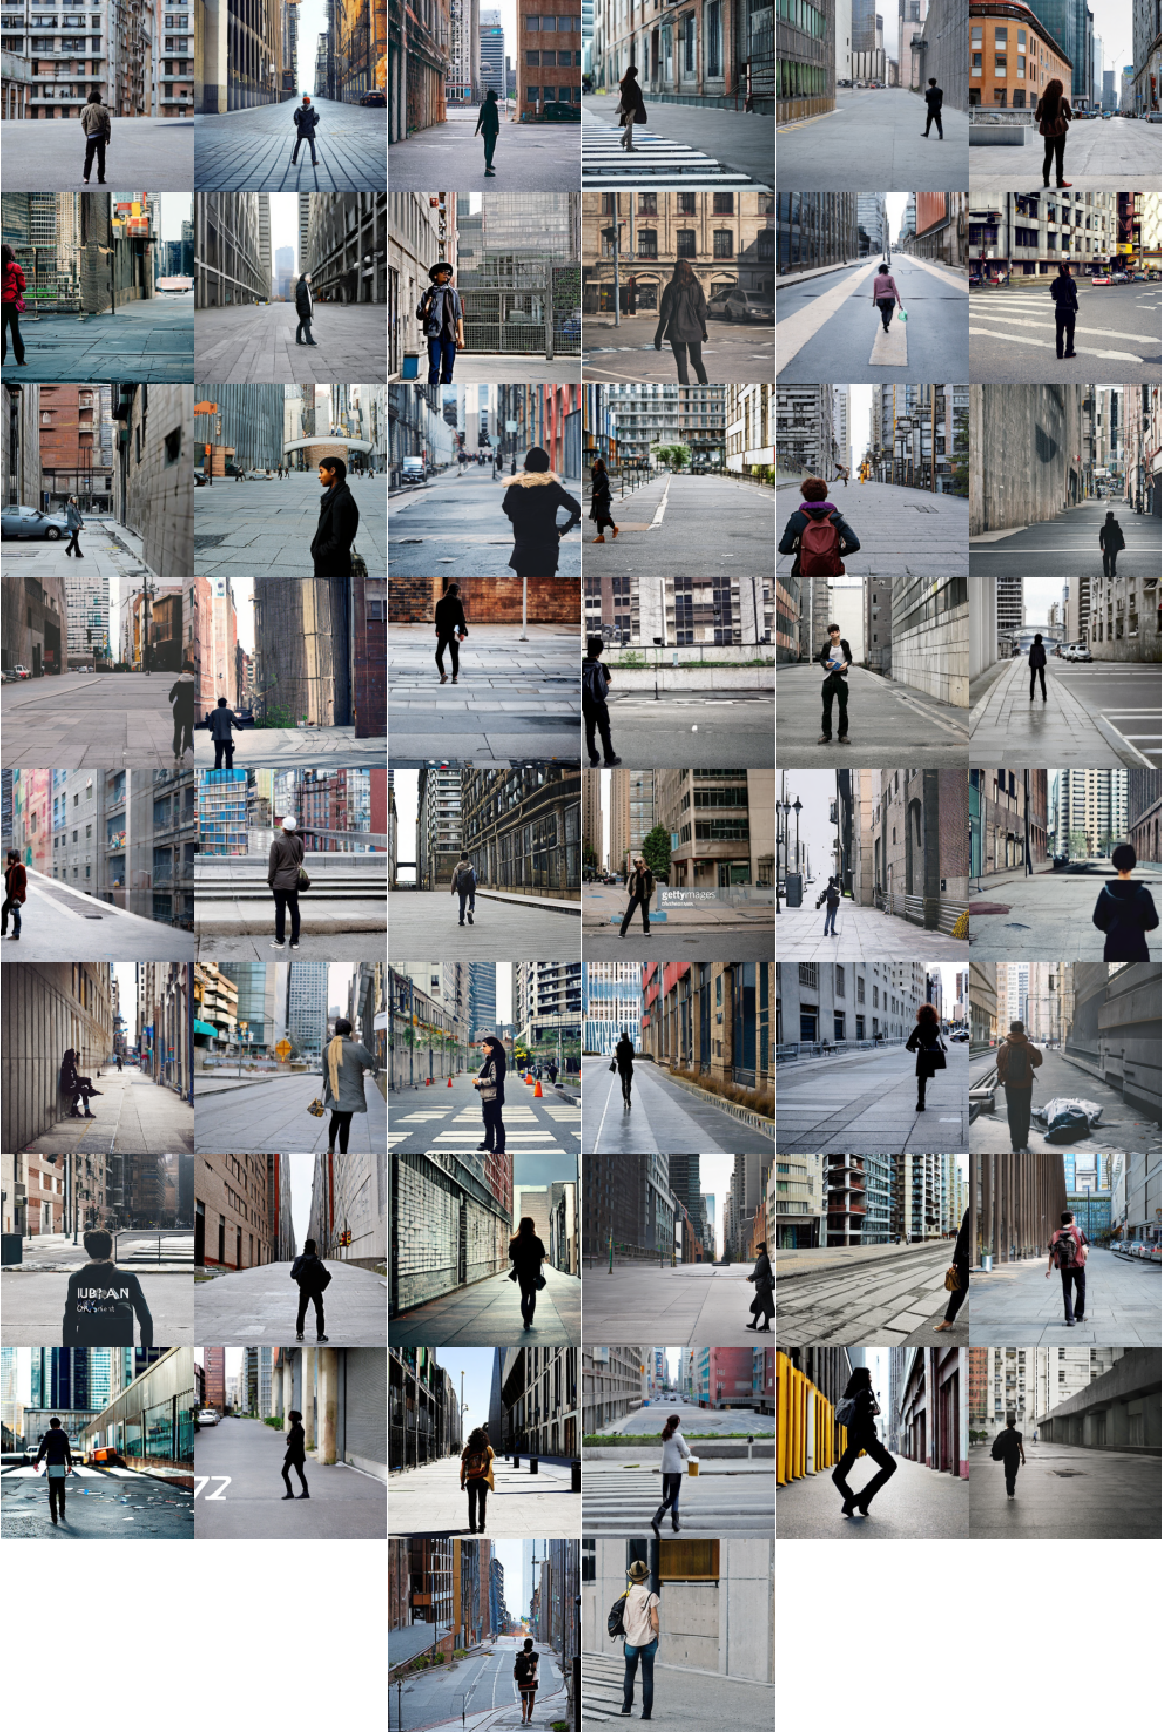
\includegraphics[width=1\columnwidth]{img/6-appendix/dataset_example_person.pdf}
    \caption[Dataset images 51-100]{Dataset images 51-100. Class ``Person''. Images generated with the prompt ``A person in an urban environment`` varying the random seed.}
    \label{fig:dataset-person}
\end{figure}


\begin{figure}
    \centering
    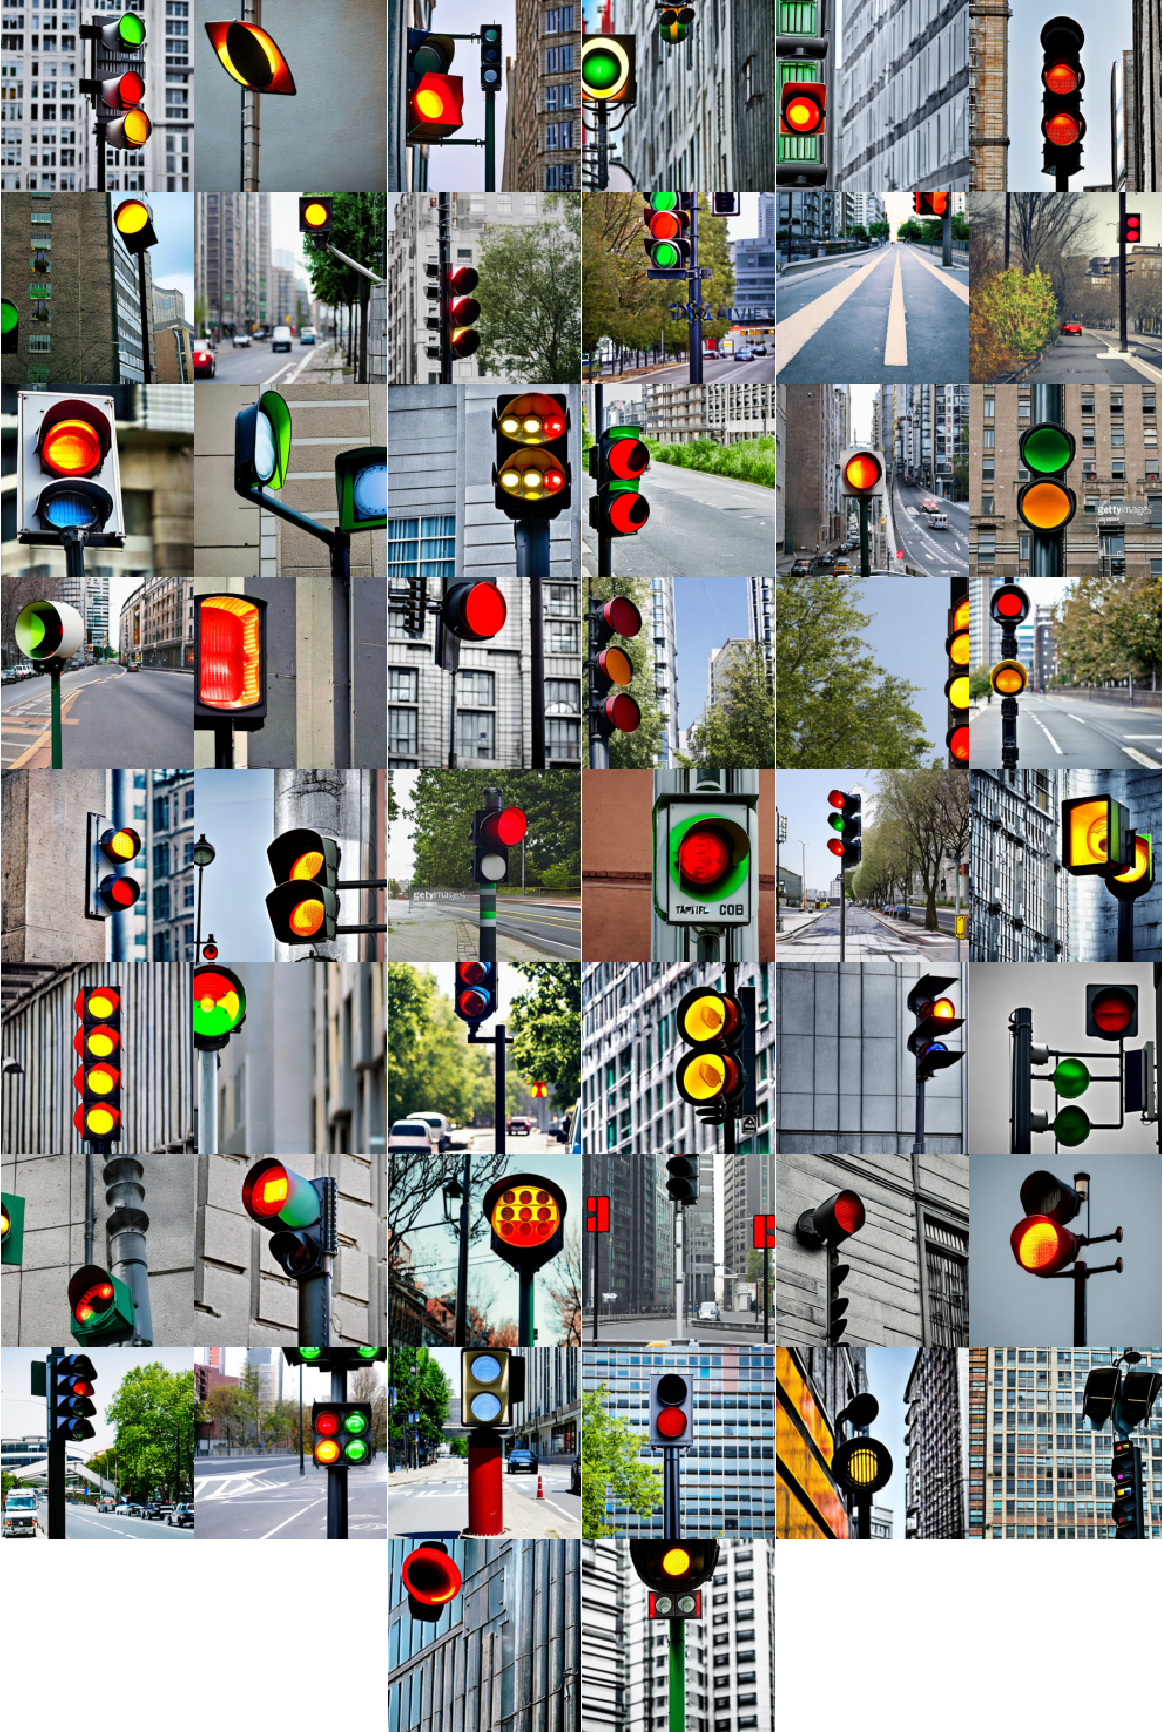
\includegraphics[width=1\columnwidth]{img/6-appendix/dataset_example_traffic light.pdf}
    \caption[Dataset images 101-150]{Dataset images 101-150. Class ``Traffic Light''.  Images generated with the prompt ``A traffic light in an urban environment`` varying the random seed.}
    \label{fig:dataset-traffic}
\end{figure}


\begin{figure}
    \centering
    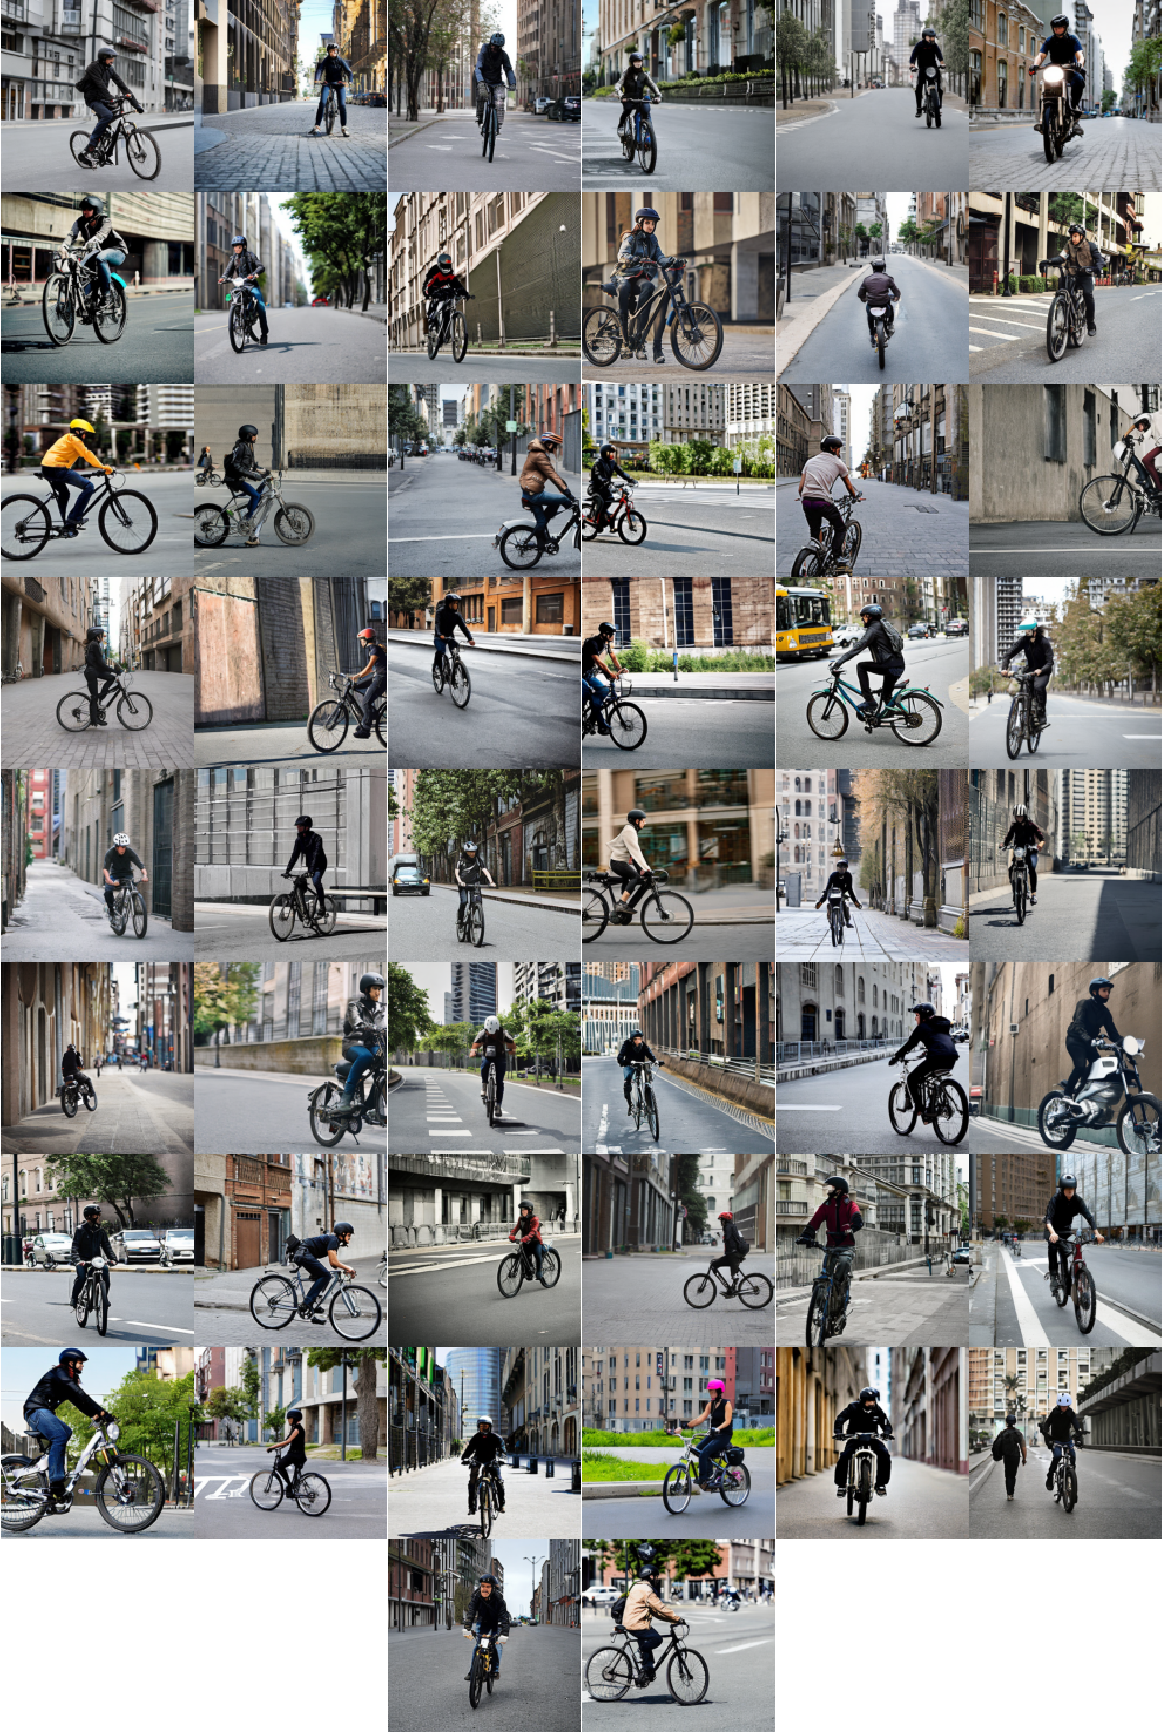
\includegraphics[width=1\columnwidth]{img/6-appendix/dataset_example_rider.pdf}
    \caption[Dataset images 151-200]{Images 151-200. Class ``Rider''.  Images generated with the prompt ``A rider in an urban environment`` varying the random seed.}
    \label{fig:dataset-rider}
\end{figure}
